\usepackage{amsmath, amsthm, amssymb}
\usepackage{tcolorbox}
\tcbuselibrary{skins, theorems, breakable}
\usepackage{tikz}
\usetikzlibrary{calc, arrows.meta,positioning}
\usepackage{geometry}
\geometry{left=3cm, right=2.5cm, top=2.5cm, bottom=2.5cm}
\tcbset{
	mymathbox/.style={
		colback=blue!5!white,
		colframe=blue!75!black,
		boxrule=1pt,
		arc=2pt,
		left=4pt, right=4pt, top=4pt, bottom=4pt
	}
}

\newtcbtheorem[auto counter, number within=chapter]{knowledge}{知识要点}%
{enhanced, colframe=blue!75, colback=blue!5, 
	boxrule=1pt, arc=3mm, fonttitle=\bfseries}{th}

\everymath{\displaystyle}

\begin{document}
	
	
	
	%-----------------------------------------------------------
	\chapter{动量与冲量}
	
	\section{导言}
	在第二章中，我们把力定义为物体间的一种相互作用，通过定义、实验等方式得到了力与加速度的关系，并引入了惯性质量，最终得到牛顿第二定律。作为本章引言，我们暂时忘记第二章的结论，换一种思考方式去审视“力”。
	
	考虑两个除运动状态外完全相同的质点。这两个质点只受到它们之间的相互作用。容易想象，任意时刻 $t$，存在这样一个参考系，在此参考系下，两质点的速度等大反向，即：
	\[ \boldsymbol{v}_1 = -\boldsymbol{v}_2 \]
	取两质点中点 $O$。根据空间反演对称性，我们断言，在相互作用的 $\Delta t$ 内，两质点的速度增量也是等值反向的：
	\[ \Delta \boldsymbol{v}_1 = -\Delta \boldsymbol{v}_2 \]
	取 $\Delta t \to 0$ 的极限，得：
	\[ \frac{d\boldsymbol{v}_2}{dt} = -\frac{d\boldsymbol{v}_1}{dt} \]
	推广至一般质点，考虑到不同质点之间的差异只能由质量（一个标量）表征，将上式改写为：
	\[ m_2 \Delta \boldsymbol{v}_2 = -m_1 \Delta \boldsymbol{v}_1 \]
	同样取 $\Delta t \to 0$ 的极限，得：
	\[ m_2 \frac{d\boldsymbol{v}_2}{dt} = -m_1 \frac{d\boldsymbol{v}_1}{dt} \]
	这揭示了一个深刻的物理事实：两个质点在相互作用时，正在相互传递着一个量。并且我们还得出，质点 1 损失多少这个量，质点 2 就得到多少这个量。
	
	最后，我们定义：力是单位时间这个量的传递，即
	\[ \text{质点 1 给质点 2 的力：} \quad \boldsymbol{f}_{12} = m_2 \frac{d\boldsymbol{v}_2}{dt} \]
	\[ \text{质点 2 给质点 1 的力：} \quad \boldsymbol{f}_{21} = m_1 \frac{d\boldsymbol{v}_1}{dt} \]
	代入上述公式得到：
	\[ \boldsymbol{f}_{12} + \boldsymbol{f}_{21} = \boldsymbol{0} \]
	我们得到了牛顿第三定律。
	
	\begin{knowledge}{力的本质}{ch3:pre-newton-core}
		本节旨在帮助读者理解重要概念：力是动量的传递。
	\end{knowledge}
	
	\section{冲量与动量定理}
	\textit{注：本节我们主要考虑质点的动量，及作用在质点上力的冲量。}
	
	\vspace{1em} 
	\noindent 对于每个质点，定义其动量为质量与速度的乘积，即：
	\[ \boldsymbol{p} = m\boldsymbol{v} \]
	\noindent 由导言的分析，或由牛顿第二定律的微分形式，可得：
	\[ \boxed{\boldsymbol{F} = \frac{d\boldsymbol{p}}{dt}} \]
	
	\begin{knowledge}{关于牛顿第二定律的思考}{ch3:second-law-essence}
		注意：$\boldsymbol{F} = d\boldsymbol{p}/dt$ 才是牛顿第二定律的更本质形式。事实上，我们无法直接通过 $\boldsymbol{F}=m\boldsymbol{a}$ 得到 $\boldsymbol{F}=d\boldsymbol{p}/dt$，因为这种推导只在 $m$ 为定值时才成立。要注意到：在 $\boldsymbol{F}=d\boldsymbol{p}/dt$ 中，质点的质量是可能变化的。
	\end{knowledge}
	
	\noindent 对 $\boxed{{F} = d\boldsymbol{p}/dt}$ 进行变形：
	\[ \boldsymbol{F}dt = d\boldsymbol{p} \]
	两边积分：
	\[ \int_{t_1}^{t_2} \boldsymbol{F} dt = \boldsymbol{p}_2 - \boldsymbol{p}_1 \]
	
	\noindent 定义冲量 [$\boldsymbol{I} = \int_{t_1}^{t_2} \boldsymbol{F} dt$]。
	
	\noindent 可以看出，冲量是力对时间的累积量，同时冲量也是矢量。利用冲量定义，我们得出动量定理：
	\[ \boxed{\boldsymbol{\boldsymbol{I} = \boldsymbol{p}_2 - \boldsymbol{p}_1 = \Delta \boldsymbol{p}}} \]
	由于上述公式均为矢量式，我们也可以写成分量形式：
	\[ I_x = \Delta p_x, \quad I_y = \Delta p_y, \quad I_z = \Delta p_z \]
	
	\begin{knowledge}{平均力的计算}{ch3:average-force}
		我们可以通过动量定理算出平均力，即 $\bar{\boldsymbol{F}} = \frac{\Delta \boldsymbol{p}}{\Delta t}$。
	\end{knowledge}
	
	\subsection*{常见误区}
	\begin{enumerate}
		\item \textbf{忽视矢量性：} 在处理反弹、斜碰等问题时，未建立坐标系进行矢量分解，直接做标量加减导致方向错误。
		\item \textbf{混淆变化量概念：} \\
		动量变化量的大小：$|\boldsymbol{\Delta p}| = |\boldsymbol{p}_2 - \boldsymbol{p}_1|$（矢量差的模）；\\
		动量大小的变化量：$\Delta|\boldsymbol{p}|  = |\boldsymbol{p}_2| - |\boldsymbol{p}_1|$（标量差）。二者通常不相等。
	\end{enumerate}
	
	\vspace{1em}
	\noindent\textbf{例题 3.2：} 喷泉中的水柱把一重为 $W$ 的桶顶在空中。已知水以恒定速率 $v_0$、恒定质量增率（单位时间喷出的质量）$Q$ 从地下射向空中，并假设水与桶撞击后以原速率、相反方向反弹，求桶可稳定停留的高度。
	
	\noindent\textbf{解答：}
	设桶可稳定停留的高度为 $h$，水柱到达此高度时与桶撞击前的速率为 $v$。根据竖直上抛运动规律，有：
	\[ v = \sqrt{v_0^2 - 2gh} \]
	在 $\Delta t$ 时间内，撞击桶的水质量为 $\Delta m = Q \Delta t$。规定竖直向上为正方向，对这部分水列动量定理：
	\[ F_{\text{水}} \Delta t = \Delta p = \Delta m (-v) - \Delta m v = -2v \Delta m \]
	得到桶对水的作用力 $F_{\text{水}}$ 为：
	\[ F_{\text{水}} = -2v \frac{\Delta m}{\Delta t} = -2vQ \]
	考虑到作用力等于反作用力，水对桶的冲击力 $F$ 大小为 $F = 2vQ$，方向竖直向上。
	当桶稳定时受力平衡，令 $F = W$，得到：
	\[ 2Q\sqrt{v_0^2 - 2gh} = W \]
	两边平方并解得桶可稳定停留的高度 $h$ 为：
	\[ h = \frac{v_0^2}{2g} - \frac{W^2}{8gQ^2} \]
	
	\vspace{1em}
	\section{质点组动量变化定理}
	\noindent 对系统每一个质点 $i$，有：
	\[ \boldsymbol{F}_{\text{外},i} + \boldsymbol{F}_{\text{内},i} = \frac{d\boldsymbol{p}_i}{dt} \]
	\\其中，$\boldsymbol{F}_{\text{外},i}$ 表示第 $i$ 个质点受到的合外力，$\boldsymbol{F}_{\text{内},i}$ 表示第 $i$ 个质点受到的合内力。
	\\
	\noindent 由牛顿第三定律，内力之和恒为零：
	\[ \sum \boldsymbol{F}_{\text{内},i} = \boldsymbol{0} \]
	于是得到：
	\[ \boxed{\sum \boldsymbol{F}_{\text{外},i} = \frac{d\boldsymbol{P}}{dt}} \]
	其中 $\boldsymbol{P} = \sum \boldsymbol{p}_i$，为质点组总动量。
	
	由上面的推导，我们能够得出质点系的一些性质：
	\begin{enumerate}
		\item 质点系内力冲量为 0，内力不能改变质点组的总动量。即便是系统内部剧烈的内力交互（如内爆、摩擦），也不会改变系统总动量。
		\item 只有外力才可能改变质点组动量。
	\end{enumerate}
	
	\noindent\textbf{例题 3.3：} 质量分别为 $m_1$、$m_2$ 和 $m_3$ 的三个质点 A、B 和 C 位于光滑的水平桌面上，用已拉直的不可伸长的柔软轻绳 AB 和 BC 连接，$\angle ABC = \pi - \alpha$。今有一冲量为 $I$ 的冲击力沿 BC 方向作用于质点 C，求质点 A 开始运动时的速度。
	
	\noindent\textbf{解答：}
	设冲击后 A, B, C 速度大小分别为 $v_A, v_B, v_C$。
	对 ABC 系统，根据质点组动量定理，在沿 BC 方向与垂直 BC 方向分别列式：
	
	\vspace{1em}
	\begin{center}
		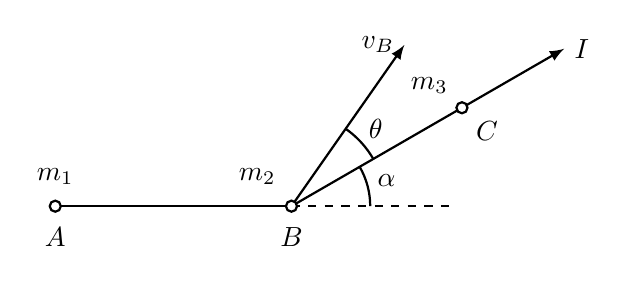
\begin{tikzpicture}[>=latex, thick]
			\coordinate (A) at (0, 0);
			\coordinate (B) at (3, 0);
			\coordinate (C) at ($(B) + (30:2.5)$);
			\draw (A) -- (B);
			\draw (B) -- (C);
			\draw[dashed] (B) -- ++(2, 0);
			\draw[->] (B) -- ($(B) + (55:2.5)$) node[left] {$v_B$};
			\draw[->] (C) -- ($(C) + (30:1.5)$) node[right] {$I$};
			\draw ($(B) + (1, 0)$) arc (0:30:1);
			\node at ($(B) + (15:1.25)$) {$\alpha$};
			\draw ($(B) + (30:1.2)$) arc (30:55:1.2);
			\node at ($(B) + (42.5:1.45)$) {$\theta$};
			\filldraw[fill=white, draw=black] (A) circle (2pt) node[below=4pt] {$A$} node[above=4pt] {$m_1$};
			\filldraw[fill=white, draw=black] (B) circle (2pt) node[below=4pt] {$B$} node[above left=4pt and 2pt] {$m_2$};
			\filldraw[fill=white, draw=black] (C) circle (2pt) node[below right=2pt] {$C$} node[above left=2pt] {$m_3$};
		\end{tikzpicture}
	\end{center}
	\vspace{1em}
	
	\begin{align*}
		\text{沿 BC 方向：} \quad & I = m_1 v_A \cos\alpha + m_2 v_B \cos\theta + m_3 v_C \\
		\text{垂直 BC 方向：} \quad & 0 = -m_1 v_A \sin\alpha + m_2 v_B \sin\theta
	\end{align*}
	考虑到绳子不可伸长的约束条件：
	\begin{align*}
		\text{沿 AB 绳方向：} \quad & v_A = v_B \cos(\alpha + \theta) \\
		\text{沿 BC 绳方向：} \quad & v_C = v_B \cos\theta
	\end{align*}
	由上述四式联立。先将速度约束代入动量方程中消去 $v_C$ 和 $\theta$，经过代数化简可解得质点 A 的速度：
	\[ v_A = \frac{I m_2 \cos\alpha}{m_2(m_1 + m_2 + m_3) + m_1 m_3 \sin^2\alpha} \]
	\textit{注：本题也可以不用质点组动量定理分析，感兴趣的读者可自行研究其他解法。}
	
	\section{动量守恒定律}
	\noindent 对于一个质点组，无论其内力如何作用，只要合外力为 0，就能保证：
	\[ \frac{d\boldsymbol{P}}{dt} = \boldsymbol{0} \]
	其中 $\boldsymbol{P}$ 是质点组总动量。
	
	\noindent 这说明，$\boldsymbol{P}$ 不随时间变化，即 $\boldsymbol{P}$ 必定为一个不变的常矢量。
	
	\noindent\textbf{说明：}
	\begin{enumerate}
		\item 由动量定理的分量式，若质点组在某一方向（以 $x$ 方向为例）合力为零，仍然有 $P_x = \text{常数}$。
		\item 动量守恒定律是一个极其普适的定律。无论是低速宏观物体的碰撞，还是高速微观粒子的裂变，动量守恒均成立。
		\item 若满足以下特殊情况，可认为质点组总动量近似守恒：
		\begin{itemize}
			\item 外力的大小远小于内力，如外力有上限（如滑动摩擦力），而内力极大（如二体碰撞时的冲击力）。
			\item 外力作用时间 $\Delta t \to 0$。例如包含重力或摩擦力的问题。此时由于 $\Delta t \to 0$，冲量 $F_{\text{外}}\Delta t \to 0$，故可认为系统动量近似守恒。
		\end{itemize}
	\end{enumerate}
	%---------------------------------------------------
	
	
	
\end{document}
